\chapter{Introduction}
\section{Polynomial constraint solving}
{\em Polynomial constraint solving} is a task of computing an assignment of variables to real/integer numbers 
that satisfies given polynomial inequalities/equations. If such an assignment exists, the constraint is said to be satisfiable (SAT) and the assignment is called SAT instance; otherwise we mention it as unsatisfiable (UNSAT). 
\begin{example} \label{examp:unsat-example}
$x^2 + y^2 < 1 \wedge xy > 1$ is an example of an UNSAT constraint. While the set of satisfiable points for the first inequality ($x^2 + y^2 < 1$) is the read circle in Figure \ref{fig:unsat-example}, the set for the second one is the green area in the figure. Because these two areas do not intersect, the conjunction of two equalities is UNSAT.
\end{example}

\begin{figure}[ht]
%\begin{minipage}[b]{1.0\linewidth}
\centering
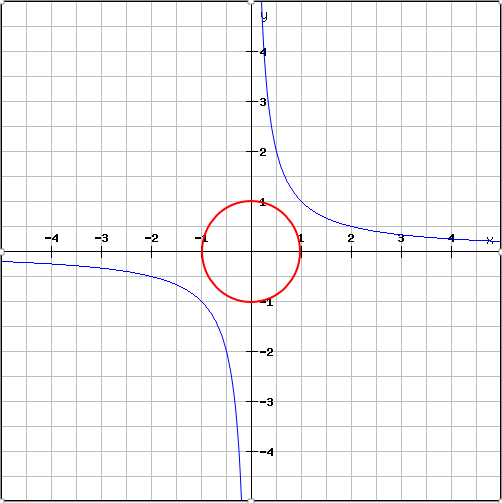
\includegraphics{UNSAT-example.png} 
\caption{Example of UNSAT constraint} 
\label{fig:unsat-example} 
%\end{minipage}
\end{figure} 

\begin{example} \label{examp:sat-example}
Figure~\ref{fig:sat-example} illustrates the satisfiability of the constraint: $x^2 + y^2 < 4 \wedge xy > 1$. Any point in the purple area is a SAT instance of the constraint, e.g. $(1.5, 1)$.
\end{example}

\begin{figure}[ht]
%\begin{minipage}[b]{1.0\linewidth}
\centering
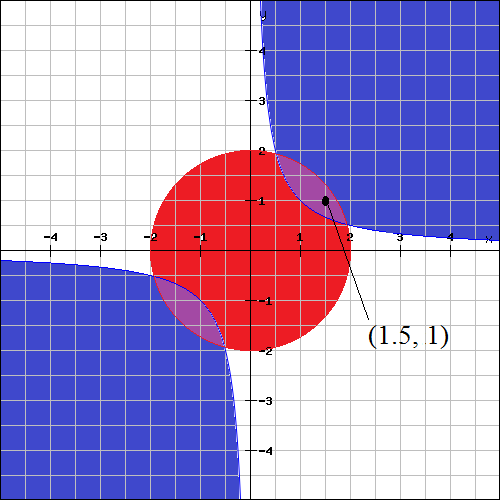
\includegraphics{SAT-example.png} 
\caption{Example of SAT constraint} 
\label{fig:sat-example} 
%\end{minipage}
\end{figure} 

%For instance, $\exists x y. -y^2 + (x^2 - 1) y - 1 > 0 \wedge -x^2 - y^2 + 4 > 0$ is 
%such an example. This is an easy formula, but proving its satisfiability and 
%showing a satisfiable instance (e.g., $x = 1.8$, $y=0.9$) are not so easy.  
%its satisfiability and a satisfiable instance 
%(e.g., $x = 1.8$, $y=0.9$) are not so easy.  		
%
Solving polynomial constraints has many application in Software Verification, such as 
\begin{itemize}
\item {\bf Locating roundoff and overflow errors}, 
which is our motivation~\cite{Ngoc:2009:ORE:1685167.1685421,Ngoc:2010:CRE:1858996.1859056}
%DSP decorders in practice are defined by reference algorithms in C using floating point arithmetic. 
%In embedded systems, often it is replaced with fixed point arithmetic, 
%which may cause visible noises. 
%and locating such roundoff error source is not easy. 
%For instance, consider DSP decoder like mpeg4. Usually, the decoder definition is given by a reference 
%algorithm in C, which uses floating point number. 
%In an embedded system, it is tempting to replace floating 
%point into fixed point numbers. However, naive replacement would cause 

\item {\bf Automatic termination proving}, 
which reduces termination detection to finding a suitable ordering~\cite{Lucas:2008:CCS:1361735.1361760}, 
e.g., \TTTT~\footnote{\url{http://cl-informatik.uibk.ac.at/software/ttt2/}}, 
Aprove~\footnote{\url{http://aprove.informatik.rwth-aachen.de}}. 
%as a solution of polynomial constraints. 

\item {\bf Loop invariant generation}. 
Farkas's lemma is a popular approach in linear loop invariant generation~\cite{Colon}, 
and is reduced to degree $2$ polynomials. 
%matrix multiplications. 
%degree $2$ polynomial constraints. 
%Farkas's lemma uses products of matrices, and it requires solving polynomial constraints of degree 2.
Non-linear loop invariant~\cite{Sankaranarayanan:2004:NLI:982962.964028} requires more complex polynomials.

\item {\bf Hybrid system}. SMT for QF\_NRA are often used as backend engines~\cite{Sankaranarayanan04constructinginvariants}. 

\item {\bf Mechanical contrnol design}. 
PID control is simple but widely used, and designing parameters is 
reduced to polynomial constraints~\cite{control}. 
%Fujitsu used polynomial constraints solving to design PID control of HDD head movement
\end{itemize}	

\section{Existing approaches}
Although solving polynomial constraints on real numbers is decidable~\cite{tarski}, current methodologies have their own pros and cos. They can be classified into the following categories: 
\begin{enumerate}
\item \textbf{Quantifier elimination by cylindrical algebraic decomposition (QE-CAD)} ~\cite{qecad} 
is a complete technique, and 
is implemented in Mathematica, Maple/SynRac, Reduce/Redlog, QEPCAD-B, and recently 
in
Z3 4.3 (which is referred as nlsat in~\cite{Jovanovic13}).
Although QE-CAD is precise and detects beyond SAT instances (e.g., SAT regions), 
scalability is still challenging, since it is DEXPTIME. 
%Since QE-CAD is DEXPTIME wrt the number of variables, 

\item \textbf{Virtual substitution (VS)}. ~
SMT-RAT toolbox \cite{smtrat}\cite{vssmt} combines 
VS, incremental DPLL, and %less lazy and 
eager theory propagation. 
Z3 (version 3.1), the winner of QF\_NRA in SMT competition 2011, 
combines VS, ICP, and linearization.

\item \textbf{Bit-blasting}. ~Bit-blasting in bounded bit width is often used in SMTs for QF\_NIA. 
UCLID~\cite{uclid} reduces the number of bits (i.e., narrowing bounds for SAT instances) 
as an under-approximation, and removes clauses as an over-approximation. 
They refine each other, which shares a similar sprit with {\bf raSAT} loop. 
MiniSmt~\cite{minismt}, the winner of QF\_NRA in SMT competition 2010, 
applies it for rational numbers with symbolic representations for prefixed algebraic numbers. 
MiniSmt can show SAT quickly with small degree polynomials, but due to the bounded bit encoding, 
it cannot conclude UNSAT.
Bit-blasting also suffers a lot when the degree of polynomials increases. 

\item \textbf{Linearization}. ~
CORD \cite{cord} uses another linearization, called 
CORDIC (COrdinate Rotation DIgital Computer) for real numbers. 
Both Barcelogic and CORD apply Yices for solving linear constraints.
Linearization also suffers a lot when the degree of polynomials increases. 

\item \textbf{Interval Constraint Propagation} 
which are used in SMT solver community, e.g., {\bf iSAT3}~\cite{isat}, 
{\bf dReal}~\cite{dRealCADE13}, and RSOLVER~\cite{rsolver}. 
ICP is based on over-approximation by interval arithmetics, and iteratively refines by
interval decompositions. 
It is practically often more efficient than algebraic computation 
with weaker theoretical completeness. 
\end{enumerate}

\section{Proposed Approach and Contributions}
Our aim is an efficient decision method for solving polynomial constraint. We combine ICP with Grobner basis method in order to solve the following cases.
\subsection{Inequalities}
Constraints with inequalities can be categorized into four cases:
\begin{enumerate}
\item \textbf{SAT with without touching}
\begin{figure}[ht]
%\begin{minipage}[b]{1.0\linewidth}
\centering
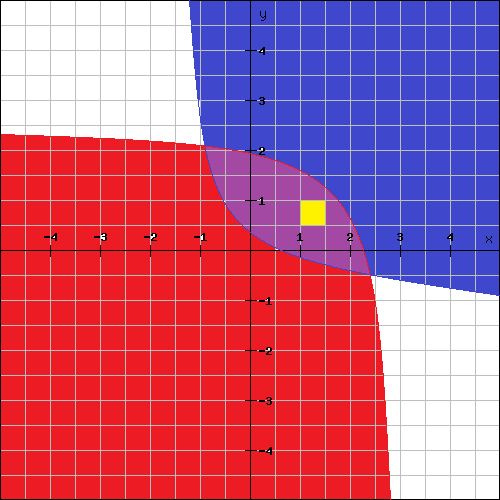
\includegraphics{SAT-withoutTouching.png} 
\caption{SAT without touching dectected by ICP} 
\label{fig:sat-withoutTouching} 
%\end{minipage}
\end{figure} 

\item \textbf{SAT/UNSAT with touching}
\begin{figure}[ht]
%\begin{minipage}[b]{1.0\linewidth}
\centering
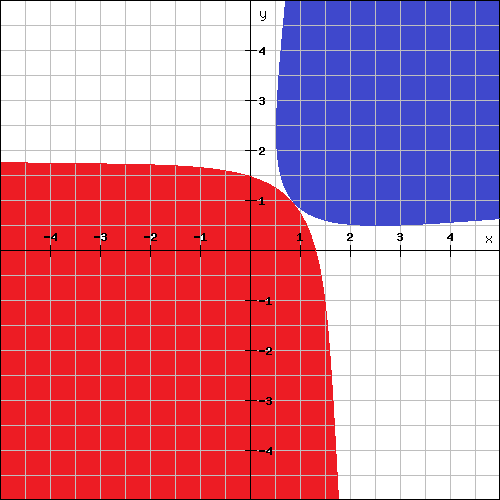
\includegraphics{SAT-touching.png} 
\caption{SAT(UNSAT) detected by Grobner basis method} 
\label{fig:sat-touching} 
%\end{minipage}
\end{figure} 

\item \textbf{UNSAT without touching}
\begin{figure}[ht]
%\begin{minipage}[b]{1.0\linewidth}
\centering
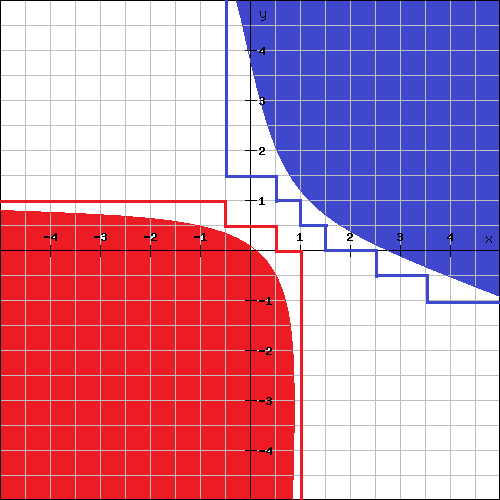
\includegraphics{UNSAT-withoutTouching.png} 
\caption{UNSAT detected by ICP} 
\label{fig:unsat-withoutTouching} 
%\end{minipage}
\end{figure} 
\end{enumerate}
$\exists x_1 \in (a_1,b_1) \cdots x_n \in (a_n,b_n) . \wedge_{i} f_i > 0$, 
\begin{itemize}
\item If $\exists x_1 \in (a_1,b_1) \cdots x_n \in (a_n,b_n) . \wedge_{i} f_i > 0$ is SAT, 
ICP eventually detects it. 
\item If $\exists x_1 \in [a_1,b_1] \cdots x_n \in [a_n,b_n] . \wedge_{i} f_i \geq 0$ is UNSAT, 
ICP eventually detects it
\end{itemize}
under the assumptions of {\em fair} decomposition and bounded intervals. 
\begin{figure}[ht]
%\begin{minipage}[b]{1.0\linewidth}
\centering
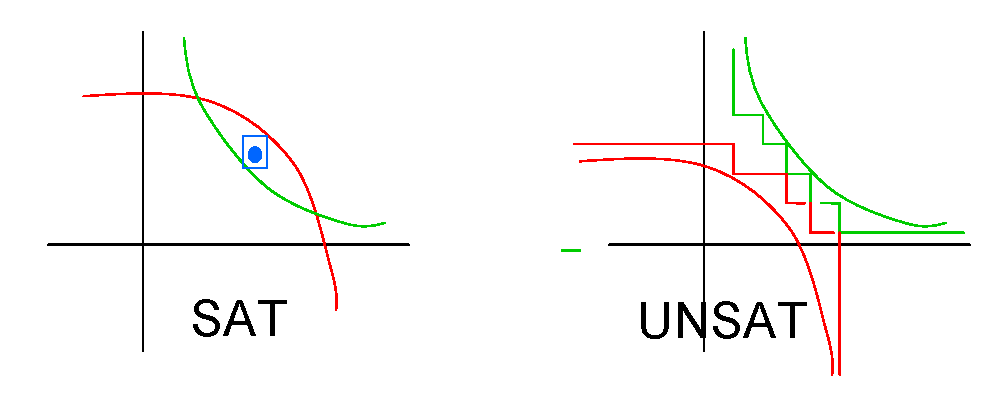
\includegraphics[height=1.2in,width=3.4in]{FigCompleteness.eps} 
\caption{SAT and UNSAT detection by ICP} 
\label{fig:complete} 
%\end{minipage}
\end{figure} 

The boundary part is reduced to polynomial equality checking, 
which would be solved algebraic methods, like Groebner basis. 
Alternatively, by loosening equality to $\delta$-equality, 
$\delta$-completeness is obtained~\cite{dRealIJCAR12,dRealLICS12}. 

This paper presents an SMT solver {\bf raSAT} for polynomial inequality. 
It consists of a simple iterative approximation refinement, called {\bf raSAT} {\em loop}, 
which is an extension of the standard ICP with testing to accelerate SAT detection. 
Two approximation schemes consist of interval arithmetic (over-approximation) and 
testing (under-approximation), to accelerate SAT detection. 
If both fails, input intervals are refined by decomposition. 
%
Compared to typical ICPs, {\bf raSAT} 
\begin{itemize}
\item introduces testing (as an under-approximation) to accelerate SAT detection, 
\item applies various interval arithmetic, e.g., Affine intervals~\cite{Stolfi03,ngocase,tapas12}, 
which enables to analyze the effects of input values, and 
\item SAT confirmation step by an error-bound guaranteed floating point package {\bf iRRAM}\footnote{% 
\tt http://irram.uni-trier.de}, to avoid soundess bugs caused by roundoff errors. 
\end{itemize}
This design is more on SAT detection oriented, since from our preliminary experiences, 
if the target problems have several hundred variables, solvable cases in practice are 
either SAT or UNSAT with small UNSAT core. 
Thus, acceleration of SAT detection and finding UNSAT core will be keys for scalability. 

ICP is robust for larger degrees, but the number of boxes (products of intervals) to explore 
exponentially explodes when variables increase. 
Thus, design of strategies for selecting variables to decompose and boxes to explore is crucial 
for efficiency. Our strategy design is, 
\begin{itemize}
\item a box with more possiblity to be SAT is selected to explore, which is estimated by 
several heuristic measures, called {\em SAT likelyhood}, 
and the number of unsolved atomic polynomial constraints, and
\item a more influential variable is selected for multiple test cases and decomposition, 
which is estimated by {\em sensitivity}. 
\end{itemize} 
Note that {\em SAT likelyhood} and {\em sensitivity} are estimated during interval arithmetic. 
Especially, the latter can be applied only with Affine intervals. 
{\bf raSAT} also applies incremental search, which is often faster in practice. 
\begin{itemize}
\item {\bf Incremental widening}. 
Starting {\bf raSAT} loop with a smaller interval, and if it is UNSAT, enlarge the input intervals
and restart. 
\item {\bf Incremental deepening}. 
Starting with the bound that each interval will be decomposed no smaller than it. 
If neither SAT nor UNSAT is detected, take a smaller bound and restart. 
\end{itemize} 
Efficient UNSAT core and UNSAT confirmation % with error bound guaranteed floating point arithmetic 
are left for future work. 

They are compared on Zankl and Meti-Tarski benchmarks from 
QF\_NRA category of SMT-LIB\footnote{\tt http://www.smtlib.org/}. 
They are also evaluated by comparing 
{\bf Z3 4.3}\footnote{\tt http://z3.codeplex.com} and {\bf iSAT3}. 
Another advantage of {\bf raSAT} is the ease to handle mixed intergers, 
and experiments on AProVE benchmark from QF\_NIA category of SMT-LIB compares {\bf raSAT} with 
{\bf Z3 4.3}. 
Although {\bf Z3 4.3} performs the best, {\bf raSAT} shows comparable SAT detection on 
very large problems (e.g., with several hundred variables) with the combination of 
{\em SAT likelyhood} and {\em sensitivity}. 


\medskip 
{\bf raSAT} applies SAT confirmation to avoid soundness errors caused by roundoff/overflow errors. 
Another static analysis based approach is found in~\cite{SilvaTACAS12}. 
